\chapter{Archictetures for dialog}\label{architectures}


\section{1}

\section{2}

\section{3}

\section{4}

\section{Deep Reinforcent Learning}

In the paper \textit{Deep Reinforcement Learning for Dialogue Generation} \cite{Li:2016} the authors notice that since seq2seq models are trained by predicting the next sentence in a given conversation using the maximum-likelihood estimation (MLE) objective function, the model tends to generate  highly generic responses such as "\textit{I don't know}". This kind of responses creates conversation with little or no informational content. For example, the author let two agents talk and find some unsatisfactory results:

\begin{quote}
\begin{itemize}
\item[] A) how old are you?
\item[] B) I'm 16
\item[] A) 16?
\item[] B) I don't know what are you talking about.
\item[] A) You don't know what are you saying.
\item[] B) I don't know what are you talking about.
\item[] A) You don't know what are you saying.
\item[] $\dots$
\end{itemize}
\end{quote}

With that in mind the authors propose adding a rewarding signal to to guide the agent towards more meaningful responses, and formulate the dialog problem such that it is possible to model the long term influenced of a utterance. They choose the theoretical framework of reinforcement learning to achieve that.

\par This is a way to change the objective function that is being maximized during training. Instead of MLE objective, they try to learn a policy optimizing the long-term developer-defined reward from ongoing dialog simulations using policy gradient methods.

\par The authors are trying to combine two traditions of research in dialog generation, the one that sees dialog generation as a translation problem (the program should translate one utterance in a response); and the other that are focused in task oriented dialogs, an agent that utter a sentence is view as an agent that need to take action in an environment. This second tradition models the dialog task as a reinforcement learning problem. 


\par In this paper the learning system is described as follows: there are to agents A and B. They take turn talking with each other. So a dialogue can be represented as the sequence: $p_1, q_1, p_2, q_2, \dots, p_i, q_i$ where $p$ and $q$ are the sentences uttered by A and B, respectively.

\par For any agent, and \textbf{action} $a$ is a sentence. Since sentence can have any length, the action space is infinite.

\par A \textbf{state} is a pair $(p_i, q_i)$ of the previous two dialogue turns.

\par A stochastic policy $\pi(a|s)$ takes the form of an LSTM encoder-decoder $P(p_{i+1}|p_i, q_i)$.

\par The reward system in this setup have many parts. i) \textbf{Ease of answering}  the first part of the reward is the signal for \textit{forward-looking}, i.e., the agent should be punished if he produce sentences that do not move the the conversation forward. Using a set of $S$ of sentences such as 'I don't know what you are talking about', 'I have no idea', etc. and a Seq2Seq model $p_{Seq2Seq}$, a reward signal is calculated as

\begin{equation}
r_1 = - \frac{1}{N_{S}} \sum_{s\in S} \frac{1}{N_{s}} \log p_{Seq2Seq}
\end{equation}

where $a$ is an action (a sentence) $N_{S}$ is the cardinality of $S$ and $N_{s}$ is the number of tokens in the dull sentence $s$.

ii) \textbf{Information Flow} the authors penalize semantic similarity (cosine similarity) between consecutive turns form the same agent. Let $p_i$ and $p_{i+1}$ be two consecutive turns and $h_{p_{i}}$ and $h_{p_{i+1}}$ be the respective representation obtained form the encoder, them the reward signal $r_2$ is defined as the negative log of the cosine similarity:

\begin{equation}
r_2 = - \log \frac{h_{p_{i}} h_{p_{i+1}}}{||h_{p_{i}}|| ||h_{p_{i+1}}||}
\end{equation}


iii) \textbf{Semantic Coherence} the authors also consider the mutual information between the action a and previous turns in the history to ensure the generated
responses are coherent and appropriate:

\begin{equation}
r_3 = \frac{1}{N_{a}} \log p_{Seq2Seq}(a| q_i, p_i) + \frac{1}{N_{q_{i}}} \log p_{Seq2Seq}^{backward}(q_i| a)  
\end{equation}

where $p_{Seq2Seq}(a| p_i, q_i)$ denotes the probability of generating
response a given the previous dialogue utterances $[p_i, q_i]$. $p_{Seq2Seq}^{backward}(q_i| a)$ denotes the backward probability
of generating the previous dialogue utterance $q_i$ based on response $a$.

And so the reward for action $a$ is:

\begin{equation}
r(a, [p_i, q_i]) = \lambda_1 r_1 + \lambda_2 r_2 + \lambda_3 r_3
\end{equation}

where $\lambda_1 + \lambda_2 + \lambda_3 = 1$ (the authors have used $\lambda_1 = 0.25, \lambda_2 = 0.25, \lambda_3 = 0.5$.

\par First the autors have trained the Seq2Sqeq model on the OpenSubtitles dataset; the treat each turn in the dataset as a target and the concatenation of two previous sentences as source inputs. they use this trained model to train a mutial information model. This last model is the one that they use to initialize the policy model $p_{RL}$.

\par In this context an episode is a simulate conversation between two agents ($A$ and $B$). At the initial step a message from the training set is fed to $A$. Using an encoder -decoder model, $A$ encodes the message and decode a set of responses to $B$. In its turn, $B$ combines the set of immediate output of $A$ with the dialog history and using the encoder-decoder model generates a set of responses. These responses are feeded to $A$, and the process continues. Figure \ref{MDPConver} shows one visualization of this process. Each played action is considered a \textit{turn}. There are two stopping criteria: one of the agents generate dull responses like "I don't know" or two consecutive responses from the same agent are highly overlapping (i.e., they share more than $80\%$ of their words).


\begin{figure}[ht!]
\label{MDPConver}
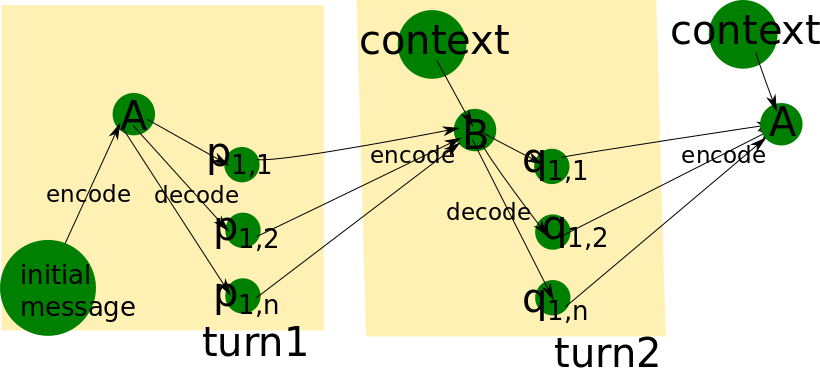
\includegraphics[width=5cm]{img/MDPconversation_placeholder.png}
\caption{MDP conversation}
\end{figure}

\par The authors use policy gradient methods to search a model to maximize the expected future reward:

\begin{equation}
J_{RL}(\vect{\theta}) = \E_{p_{RL}(a_{1:T})} \left[\sum_{i=1}^{T} R(a_i, [p_i, q_i]) \right]
\end{equation}

where $R(a_i, [p_i, q_i])$ denotes the reward resulting from action $a_i$. The gradient is estimated by the \textit{likelihood ratio trick}:

\begin{equation}
\grad{\vect{\theta}}{J_{RL}} \approx \sum_{i} \grad{\vect{\theta}}{p(a_{i} | p_{i}, q_{i})} \sum_{i=1}^{T}R(a_i, [p_{i}, q_{i}])
\end{equation}

\par Three different metrics are used: i) \textit{length of the dialog} -- average number of simulated turns; ii) \textit{degree of diversity} -- number of distinct unigrams and bigrams in generated responses; iii) \textit{human evaluation}.

\par The paper compare three models: Seq2seq, mutual information and the proposed model using reinforcement learning (RL model). The RL model have a slightly better score then the mutual information model in i) and ii). But in iii) human judges are presented with simulated conversation between the two agents, some conversation were generated by the RL model and some were generated by the mutual information model. The judges voted in which one is the better (ties are permitted).  The RL model win $72\%$ of time, lose $12\%$ of time and tie $16\%$ of time.